\documentclass[12pt,a4paper]{report}
\usepackage[utf8]{inputenc}
\usepackage[explicit]{titlesec}
\usepackage[dvipsnames]{xcolor}
\usepackage{amsmath}
\usepackage{amsfonts}
\usepackage{url}
\usepackage{amssymb}
\usepackage{makeidx}
\usepackage{graphicx}
\usepackage{tikz}
\usepackage[many]{tcolorbox}
\usepackage{standalone}
\usepackage{animate}
\tcbuselibrary{listings}
\usepackage{tabularx}
\usepackage{colortbl}
\usepackage{multicol}
\usepackage{makecell}
\usepackage{adjustbox}
\usepackage{subfig}
\usepackage{lipsum}
\usepackage{float} % Added for figure positioning

\usepackage{framed}
\usepackage{lastpage}

\usepackage{fancyhdr}
\usetikzlibrary{calc,arrows.meta,backgrounds,shapes.geometric,positioning}
\setlength{\parindent}{0pt}
\newcommand{\msymbol}[1]{\ifmmode #1 \else $#1$\fi}

\newcommand{\daemathvariable}[1]{{\normalsize \color[RGB]{100,149,237}#1}}
\newcommand{\daemathvalue}[1]{{\normalsize \color[RGB]{153,153,255}#1}}
\newcommand{\daemath}[1]{{\large \color[RGB]{0,0,0}#1}}
\newcommand{\daered}[1]{{\normalsize \color[RGB]{234,0,33}#1}}
\newcommand{\daegreen}[1]{{\normalsize \color[RGB]{0,255,65}#1}}
\newcommand{\mmathvariable}[1]{{\begingroup  \color[RGB]{100,149,237}#1 \endgroup} }
\newcommand{\mmathvalue}[1]{{\begingroup  \color[RGB]{153,153,255}#1 \endgroup} }
\newcommand{\mmath}[1]{{\begingroup  \color[RGB]{0,0,0}#1 \endgroup} }
\newcommand{\mred}[1]{{\begingroup  \color[RGB]{234,0,33}#1 \endgroup} }
\newcommand{\mgreen}[1]{{\begingroup  \color[RGB]{0,255,65}#1 \endgroup} }
\definecolor{backgroundStroke}{RGB}{0,0,0}
\definecolor{backgroundFill}{RGB}{255,255,255}
\definecolor{backgroundText}{RGB}{0,0,0}
\definecolor{bgChapter}{RGB}{91,155,213}
\definecolor{bgSection}{RGB}{222,234,246}
\definecolor{fontSubsection}{RGB}{53,124,177}
\colorlet{shadecolor}{bgChapter}

\renewcommand{\contentsname}{Contents}
\newcommand{\pbreak}{\vskip 0.5cm}
\renewcommand{\thesection}{\arabic{section}}

\newcommand{\daechapter}[1]{
  \chapter*{#1} % Create an unnumbered chapter
  \addcontentsline{toc}{chapter}{#1} % Add the chapter to the ToC
}

\newcommand{\daesection}[1]{
  \refstepcounter{section} % Increment section counter manually
  \section*{\thesection\quad #1} % Show number in title
  \addcontentsline{toc}{section}{\thesection\quad #1}
}

\newtcolorbox{ybox}{
  colback=yellow,
  colframe=yellow,
  boxrule=0pt,
  arc=0pt,
  outer arc=0pt,
  boxsep=0pt,
  left=1pt,
  right=1pt,
  top=1pt,
  bottom=1pt
}

\newtcolorbox{gbox}{
  colback=lightgray,
  colframe=lightgray,
  boxrule=0pt,
  arc=0pt,
  outer arc=0pt,
  boxsep=0pt,
  left=1pt,
  right=1pt,
  top=1pt,
  bottom=1pt
}

\pagecolor{backgroundFill}
\color{backgroundText}
\everymath{\color{backgroundText}}

\titleformat{\chapter}[display]{\normalfont\color{white} \begin {shaded*}\bfseries}{\large\chaptername~\thechapter}{20pt}{\Large#1\end{shaded*}}

\titleformat{\section}
  {\normalfont\Large\bfseries} 
  {}{0em} 
  { 
    \colorbox{bgSection}{%
      \parbox{\dimexpr\textwidth-2\fboxsep\relax}{\thesection\quad#1}
    }
  }
  
\titleformat{\subsection}
  {\color{fontSubsection}\titlerule\vspace{1ex} \normalfont\large\bfseries}
  {\thesubsection}{1em}
  {
  	\quad #1
  }
  
\titleformat{\subsubsection}
  {\color{fontSubsection}\titlerule\vspace{1ex}\normalfont\normalsize\bfseries}
  {\thesubsubsection}{1em}
  {	
  	 \quad #1   	 
  }
 
% information about the gradwork
\def\title{Incremental Performance and Quality Analysis of Hybrid Ray Tracing}
\def\subtitle{Vulkan vs DXR in Real-Time Rendering}
\def\author{De Meyer Luca}
\def\academicyear{2025-2026}


\fancyhf{}
\fancyhead[L]{\author}
\fancyfoot[L]{DAE - Graduation work 2025-2026}
\fancyfoot[R]{\thepage/\pageref{LastPage}}


\begin{document}
\pagestyle{fancy}

\begin{titlepage}
   \begin{center}
       \vspace*{1cm}
       \Huge{\title}
       \vspace{0.5cm}
       
       \Large{\subtitle}
       \vspace{1.5cm}
       
       \textbf{\author}
       \vfill
       \Large{Graduation work \academicyear}
      
     
		\begin{figure}[h]
    		\begin{minipage}[t]{0.40\textwidth}
        		\includegraphics[height=2cm]{logos/Howest_logo.png}
    		\end{minipage}\hfill
	    	\begin{minipage}[t]{0.40\textwidth}
   
   		    \centering
		        \includegraphics[height=2cm,trim=2cm 7cm 0.5cm 6cm,clip]{logos/DAE_logo.pdf}
       
    		\end{minipage}
			\vspace{0.8cm}
		\end{figure}
   \end{center}
\end{titlepage}

\tableofcontents

% -----------------------------------------------------------
% ABSTRACT & KEYWORDS
% -----------------------------------------------------------
\daechapter{Abstract {\&} Keywords}

Real-time rendering has converged on hybrid pipelines that combine rasterization with selectively applied ray tracing, yet developers still lack quantitative guidance on how to prioritize ray-traced features under fixed frame-time budgets.
While effects such as shadows, reflections, and global illumination can substantially improve visual fidelity, their performance costs and perceptual benefits vary widely across scenes, sampling strategies, and denoising configurations,
complicating engine-level decision making.
This study evaluates the incremental performance cost and visual impact of ray-traced shadows and reflections using both Vulkan Ray Tracing and DirectX Raytracing (DXR). We analyze multiple hybrid strategies—including G-buffer–guided ray generation,
adaptive sampling, and screen-space fallbacks—across three representative scenes at 1080p and 1440p resolutions, targeting real-time frame budgets on contemporary mid-range GPUs. Visual quality is assessed against a path-traced reference using perceptual
similarity metrics (LPIPS, SSIM), while GPU profiling is used to measure feature-level costs.
By combining these measurements, we derive a quality-per-millisecond metric that enables direct comparison of hybrid rendering configurations. Our results provide practical recommendations for incremental ray tracing adoption in real-time applications,
demonstrating that consistently offers the most favorable balance between perceptual quality and performance across the tested scenarios.

\begin{gbox}
\textbf{Keywords:} Real-time rendering, Hybrid Ray Tracing, Vulkan, DXR, Shadows, Reflections, Performance Analysis, Perceptual Quality, LPIPS.
\end{gbox}

% -----------------------------------------------------------
% PREFACE (Placeholder based on typical DAE structure)
% -----------------------------------------------------------
\daechapter{Preface}
\begin{ybox}
This graduation project explores incremental hybrid ray tracing strategies in real-time rendering. The goal is to provide developers practical guidance on prioritizing ray-traced features under fixed frame-time budgets.
\end{ybox}

\begin{gbox}
I would like to thank my supervisors and peers at Howest-Digital Arts and Entertainment for their guidance and feedback throughout the research process.
\end{gbox}

% -----------------------------------------------------------
% LIST OF FIGURES
% -----------------------------------------------------------
\daechapter{List of figures}
\addcontentsline{toc}{chapter}{List of figures}

% (Figures are automatically generated by LaTeX usually, but if you need manual lists as per template:)
\begin{ybox}
Figure 1: Graphics Rendering Pipeline\\
Figure 2: Geometry Processing Pipeline\\
Figure 3: Rasterization Stage
\end{ybox}

% -----------------------------------------------------------
% INTRODUCTION
% -----------------------------------------------------------
\daechapter{Introduction}
Hardware-accelerated ray tracing is now a mature feature of contemporary consumer GPUs, forming a standard component of real-time rendering pipelines across both high-end engines and commercial games. Rather than replacing rasterization,
 ray tracing is typically deployed selectively within hybrid pipelines, where it augments traditional techniques to improve lighting fidelity, visibility accuracy, and geometric correctness under strict performance constraints.

Although recent hardware generations and advanced denoising techniques have enabled real-time path-traced rendering in controlled scenarios, fully converged path tracing remains impractical for most interactive applications without aggressive
spatio-temporal reconstruction. Consequently, modern engines rely on incremental ray tracing adoption, allocating a limited ray budget to specific effects such as shadows and reflections while retaining rasterization for primary visibility and shading.

Determining how to allocate this budget presents a nontrivial optimization problem. The performance cost of individual ray-traced features varies significantly with scene complexity, sampling strategy, and acceleration structure usage,
while the resulting perceptual benefit depends heavily on lighting conditions, material properties, and denoising quality. Existing evaluations primarily focus on fully path-traced pipelines or isolated techniques, providing limited guidance
for hybrid approaches.

Furthermore, while both Vulkan Ray Tracing and DirectX Raytracing (DXR) expose similar hardware acceleration mechanisms, comparative studies at the application level—particularly for hybrid rendering workloads—remain sparse in the public literature.


\begin{gbox}
\textbf{Research Goals and Contributions:}
\begin{itemize}
    \item Quantitative measurement of incremental ray tracing costs for shadows and reflections individually and in combination.
    \item Perceptual quality analysis of different sampling rates and denoising strategies using LPIPS, SSIM metrics.
    \item Direct performance comparison of Vulkan Ray Tracing and DXR on identical hardware and workloads.
    \item Quality-per-millisecond ranking of hybrid rendering strategies (G-buffer-guided, adaptive sampling, screen-space fallbacks).
    \item Practical configuration recommendations for achieving 60 FPS targets on mid-range RTX hardware.
\end{itemize}
\end{gbox}
% -----------------------------------------------------------
% LITERATURE STUDY
% -----------------------------------------------------------
\daechapter{Literature study / Theoretical framework}
%real-time rendering
\daesection{Rasterization Fundamentals}
\begin{ybox}
Rasterization is the dominant rendering technique in real-time computer graphics, used in almost all 3D interactive applications.
The fundamental principle involves converting 3D geometry into a 2D grid of pixels. By using the GPU, which is highly optimized to rasterize millions of triangles, rasterization is fast and efficient, forming the backbone of real-time rendering.
\end{ybox}

Understanding rasterization requires a structured view of how modern GPUs transform scene data into pixels, which is formalized by the graphics rendering pipeline.


\subsection{The Graphics Rendering Pipeline}
\begin{gbox}
The graphics rendering pipeline is the fundamental framework through which a 3D scene is transformed into a 2D image for display. 
Its primary function is to generate an image from a virtual camera by processing scene geometry, materials, lighting, and other environmental parameters.
The pipeline is composed of multiple stages, each performing a specific part of the overall rendering process. 
Object positions and shapes are determined by their geometric data and transformations, while their appearance is influenced by material properties, shading models, and the scene's light sources. 
The following sections provides a brief overview of each stage, focusing on their functional roles within the pipeline.
%rewritten later
\end{gbox}

\begin{figure}[H]
\centering
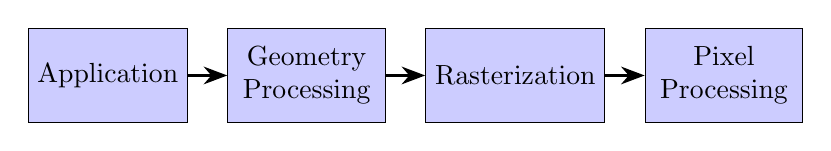
\begin{tikzpicture}[
    node distance=0.5cm,
    box/.style={rectangle, draw, fill=blue!20, minimum width=2cm, minimum height=1.2cm, align=center},
    arrow/.style={-{Stealth[length=3mm]}, thick}
]
    \node[box] (n1) {Application};
    \node[box, right=of n1] (n2) {Geometry\\Processing};
    \node[box, right=of n2] (n3) {Rasterization};
    \node[box, right=of n3] (n4) {Pixel\\Processing};
    \draw[arrow] (n1) -- (n2);
    \draw[arrow] (n2) -- (n3);
    \draw[arrow] (n3) -- (n4);
\end{tikzpicture}
\caption{Graphics Rendering Pipeline}
\label{fig:Graphics-Rendering-Pipeline}
\end{figure}

\subsection{Pipeline Stages}
\paragraph{The Application Stage:}

This stage typically executes on the CPU and provides developers with full control over rendering behavior. As a result, it can be extensively customized to suit application-specific requirements.
Decisions made during this stage—such as draw call organization, resource binding, and state changes—can significantly impact the performance of subsequent pipeline stages. At the end of the application stage,
geometry and associated data are submitted to the GPU for further processing.

\paragraph{Geometry Processing:}

 Geometry processing is divided into four distinct substages within the graphics pipeline.

\paragraph{Vertex Shading:}
The vertex shading stage is a fully programmable stage responsible for transforming vertex data and preparing per-vertex attributes for subsequent pipeline stages.
Its primary function is to compute vertex positions by transforming them from object space through world and view space into clip space using the appropriate transformation matrices.
In addition, the vertex shader evaluates and outputs any per-vertex attributes required later in the pipeline, such as normals, texture coordinates, tangents, or user-defined data.

Historically, vertex shading also performed a significant portion of lighting calculations by evaluating illumination at each vertex and interpolating the resulting color across primitives.
With modern GPUs and the widespread adoption of per-pixel shading, most lighting computations have shifted to later stages. As a result, the vertex shading stage now primarily serves as a general-purpose setup stage,
handling tasks such as geometry transformation, vertex skinning, and attribute preparation rather than direct lighting evaluation.

Every graphics pipeline includes the vertex processing stage described above; however, additional optional programmable stages may be executed on the GPU depending on both hardware capabilities and the requirements of the application.
Not all GPUs support these stages, and their use is determined by the programmer based on the desired visual fidelity and performance constraints.
\paragraph{Tesellation:}

Tessellation addresses the problem of efficiently rendering curved or highly detailed surfaces. For example, a spherical object may appear smooth when viewed from a distance but reveal its underlying triangular structure when observed up close.
One way to address this would be to increase the geometric complexity of the mesh uniformly; however, this approach wastes processing resources when high detail is unnecessary.
Tessellation enables the dynamic refinement of geometry by increasing the number of triangles only where additional detail is required.

The tessellation stage consists of three distinct substages: the hull shader, the fixed-function tessellator, and the domain shader. Geometry is initially described as a set of patches, where each patch is defined by a small number of control vertices.
The hull shader determines tessellation factors for each patch, often based on criteria such as distance from the camera or surface curvature. The tessellator then subdivides the patches into a finer set of primitives,
and the domain shader evaluates the final vertex positions of the generated geometry. This process allows the level of geometric detail to adapt dynamically based on the camera’s position relative to the surface.
\paragraph{Geometry shader:}

The geometry shader is an optional programmable stage that operates after vertex processing and primitive assembly. Unlike tessellation, which is designed for adaptive geometric refinement,
the geometry shader processes complete primitives (such as points, lines, or triangles) and can emit zero or more output primitives. While geometry shaders are more widely supported than tessellation on older hardware,
they are significantly more limited in throughput and output flexibility.

The geometry shader is commonly used for tasks such as particle expansion, procedural geometry generation, primitive amplification, and geometry-based effects that require access to entire primitives rather than individual vertices.
However, due to its relatively high performance cost and limited parallelism, the geometry shader is generally avoided in performance-critical real-time rendering pipelines and has largely been supplanted by compute shaders or alternative techniques in
modern engines.

\paragraph{Stream Output:}
Stream output is an optional pipeline feature that enables vertex or geometry shader output to be captured directly into GPU buffers for reuse in later rendering passes,
avoiding CPU readback. While useful for certain techniques such as GPU-based particle simulation or procedural geometry generation, stream output is infrequently used in modern real-time rendering pipelines and has limited relevance
to hybrid ray tracing workflows.

\paragraph{Clipping: }
Clipping is a fixed-function stage that removes or trims primitives that lie partially or entirely outside the view frustum. Geometry that falls completely outside the frustum is discarded, while primitives intersecting
the frustum boundaries are clipped to ensure that only visible portions proceed further in the pipeline. This step ensures correctness and prevents unnecessary processing in later stages.

 \paragraph{Screen Mapping: }
After clipping, vertex positions in clip space undergo perspective division, transforming them into normalized device coordinates.
These coordinates are then mapped to screen space through the viewport transformation, converting the three-dimensional scene representation into two-dimensional screen coordinates suitable for rasterization.


\begin{figure}[H]
\centering
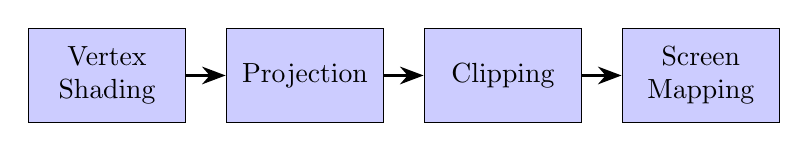
\begin{tikzpicture}[
    node distance=0.5cm,
    box/.style={rectangle, draw, fill=blue!20, minimum width=2cm, minimum height=1.2cm, align=center},
    arrow/.style={-{Stealth[length=3mm]}, thick}
]
    \node[box] (n1) {Vertex\\Shading};
    \node[box, right=of n1] (n2) {Projection};
    \node[box, right=of n2] (n3) {Clipping};
    \node[box, right=of n3] (n4) {Screen\\Mapping};
    \draw[arrow] (n1) -- (n2);
    \draw[arrow] (n2) -- (n3);
    \draw[arrow] (n3) -- (n4);
\end{tikzpicture}
\caption{Geometry Processing}\label{fig:geometry-processing}
\end{figure}

\paragraph{Rasterization Stage:} Rasterization converts screen-space primitives into fragments corresponding to pixel locations on the render target.
During this process, per-vertex attributes such as texture coordinates, normals, and colors are interpolated across each primitive. The resulting fragments are then passed to the fragment shading stage, where per-pixel operations such as shading,
texturing, and depth testing are performed.


\begin{figure}[H]
\centering
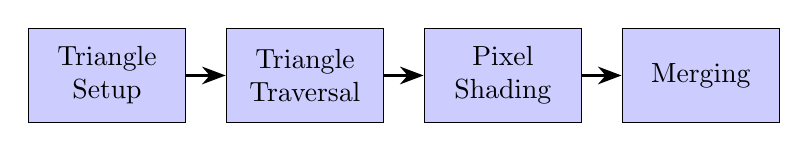
\begin{tikzpicture}[
    node distance=0.5cm,
    box/.style={rectangle, draw, fill=blue!20, minimum width=2cm, minimum height=1.2cm, align=center},
    arrow/.style={-{Stealth[length=3mm]}, thick}
]
    \node[box] (n1) {Triangle\\Setup};
    \node[box, right=of n1] (n2) {Triangle\\Traversal};
    \node[box, right=of n2] (n3) {Pixel\\Shading};
    \node[box, right=of n3] (n4) {Merging};
    \draw[arrow] (n1) -- (n2);
    \draw[arrow] (n2) -- (n3);
    \draw[arrow] (n3) -- (n4);
\end{tikzpicture}
\caption{Rasterization Stage}\label{fig:rasterization-stage}
\end{figure}
%real-time rendering
\daesection{GPU Parallelism and the Graphics Pipeline}

\subsection{GPU Parallelism Model}
Massive data parallelism

SIMT / SIMD execution

Warps / wavefronts (vendor-agnostic language)

\subsection{Fixed-Function vs Programmable Stages}
Fixed-function: rasterizer, clipping, interpolation

Programmable: shaders, compute
\subsection{Memory Hierarchy \& Bandwidth}
Registers, shared memory, caches

Global memory and bandwidth pressure

Render targets and G-buffers
\subsection{Asynchronous \& Compute Capabilities}
Async compute

Overlapping raster + ray workloads

Compute shaders replacing geometry stages

\daesection{Rendering Pipeline Variants}
%learn opengl, deferred-shading chapter
\subsection{Forward Rendering}
In a forward rendering pipeline, scene geometry is rasterized and shaded in a single pass, with lighting computations performed directly during fragment shading.
Each visible fragment evaluates the contribution of relevant light sources to produce its final color.
This approach is conceptually simple and aligns closely with the traditional graphics pipeline, making it straightforward to implement and well suited for scenes with a limited number of lights.

However, the computational cost of forward rendering scales with both the number of fragments and the number of active light sources.
In scenes with many lights, each fragment must evaluate multiple lighting equations, resulting in increased shading cost and reduced performance.
Furthermore, forward rendering is susceptible to high overdraw in scenes with significant depth complexity, where multiple fragments may be shaded before being rejected by depth testing.

Despite these limitations, forward rendering handles transparency naturally, as shading is performed in depth-sorted order.
This makes it well suited for effects such as particles and alpha-blended geometry, which remain challenging for alternative pipeline designs.

Modern variants such as Forward+ mitigate these costs through screen-space light culling, though lighting computations remain tightly coupled to fragment shading.
\subsection{Deferred Rendering}
To address the scalability limitations of forward rendering in scenes with many dynamic light sources, deferred rendering separates geometry processing from lighting evaluation.
Instead of computing lighting during rasterization, deferred rendering divides the pipeline into two distinct passes: a geometry pass and a lighting pass.\\

During the geometry pass, the entire scene is rendered once, and relevant per-fragment attributes—such as world-space position or depth, surface normals, albedo, and material properties—are written to a set of render targets collectively referred
to as the G-buffer.
Depth testing is performed during this stagealternatively, the programmer may employ a depth pre-pass executed prior to the G-buffer pass.
A depth pre-pass ensures that only the closest visible fragment at each pixel contributes to the stored G-buffer data, reducing overdraw and unnecessary fragment shading.\\

In the subsequent lighting pass, lighting calculations are performed in screen space by sampling the G-buffer.
Because lighting is evaluated only for visible fragments, the cost of shading scales primarily with screen resolution rather than scene complexity.
This makes deferred rendering particularly well suited for scenes with a large number of dynamic light sources.\\

Despite its advantages, deferred rendering introduces several challenges.
Storing multiple high-resolution render targets significantly increases memory usage and bandwidth requirements.
Additionally, traditional deferred pipelines do not natively support hardware multisample anti-aliasing (MSAA), and handling transparency is non-trivial due to the decoupling of geometry and lighting.
As a result, deferred rendering pipelines often combine multiple techniques to address these limitations.

\subsubsection{G-Buffer}
The G-buffer is a collection of screen-space render targets that store per-fragment geometric and material information required for subsequent lighting evaluation.
Typical contents include:

\begin{itemize}
    \item \textbf{World-space position vectors:} Used to reconstruct the 3D location of each fragment for lighting and shading calculations.
    \item \textbf{Surface normals:} Required for accurate lighting, reflections, and shading computations.
    \item \textbf{Albedo (diffuse color):} Stores the base color of the surface without lighting applied.
    \item \textbf{Additional material properties (optional):} Such as roughness, metallicity, and specular intensity for physically based rendering workflows.
\end{itemize}

These buffers collectively allow the lighting pass to operate independently of scene geometry, enabling deferred shading and efficient evaluation of multiple light sources.


\subsubsection{Lighting Pass}
The lighting pass operates entirely in screen space, reconstructing surface properties from the G-buffer to compute lighting contributions for each visible pixel.
Because only the closest visible fragments are stored in the G-buffer, lighting computations are performed solely for pixels that will contribute to the final image, improving performance in scenes with high depth complexity.
Multiple light sources can be evaluated in this pass without re-rendering the geometry, making deferred rendering particularly advantageous for scenes with numerous dynamic lights.


\daesection{Ray Tracing \& Hybrid Strategies}
% using ray tracing gems 1 , chapter 1-2
\subsection{Ray Tracing Fundamentals}
Ray tracing is a rendering technique that simulates the physical behavior of light by tracing rays through a scene. 
The process begins with \emph{ray casting}, where rays are emitted from the camera and intersect with scene geometry to determine visible surfaces. 
From each intersection point, secondary rays can be cast toward light sources to evaluate shadowing, or recursively into the scene to capture reflections and refractions.

To limit computational cost, a maximum recursion depth, or \emph{bounce limit}, is typically imposed. The resulting tree of rays is evaluated in reverse order, propagating light contributions back to the camera to compute the final shading.

Several variants of ray tracing exist:
\begin{itemize}
    \item \textbf{Whitted (classical) ray tracing:} Assumes perfectly specular and smooth surfaces, with light sources represented as discrete directions. Each intersection generates reflection, refraction, and shadow rays as needed.
    \item \textbf{Cook or stochastic ray tracing:} Introduces probabilistic sampling at each intersection, allowing multiple rays to be emitted per node to produce effects such as glossy reflections, soft shadows, and indirect illumination.
    \item \textbf{Path tracing:} Uses stochastic sampling to estimate the full light transport equation. Rays are traced from the camera, and at each intersection, incoming light directions are sampled according to the surface’s material properties.
     This approach captures global illumination, including multiple bounces, soft shadows, and color bleeding.
\end{itemize}

\subsection{What is a Ray?}
A ray is a three-dimensional half-line, usually defined by an \daemathvariable{origin point O} and a \daemathvariable{direction vector D}. 
Unlike a 2D line, which can be expressed as \daemath{y = mx + b}, a 3D ray can be written in parametric form:\\

\daemath{P(t) = O + t D}, with $t \ge 0$\\

%cant use greater than  symbol in daemath?
Here, \daemathvariable{P(t)} denotes a point along the ray, \daemathvariable{t} is a scalar parameter, 
\daemathvariable{O} is the \emph{ray origin}, and \daemathvariable{D} is the \emph{ray direction}. 
The condition \daemathvariable{t} $\ge$ \daemathvariable{0} ensures the half-line extends only in the direction of D.\\

%need the ray segement from ray tracing gems chapter 2 here somewhere
\paragraph{Ray Types:}
Rays are often categorized depending on their role in rendering:
\begin{itemize}
    \item \textbf{Primary rays:} start at the camera, passing through pixels to determine visible surfaces.
    \item \textbf{Shadow rays:} shot from surface intersections to light sources to determine occlusion.
    \item \textbf{Reflection rays:} generated from reflective surfaces along mirror directions.
    \item \textbf{Refraction rays:} travel through transparent or refractive surfaces according to Snell’s law.
    \item \textbf{Eye rays vs. light rays:} primary rays are “eye rays” from the camera, while secondary rays can be considered “light rays” contributing to illumination.
\end{itemize}
In recursive ray tracing, rays are typically traced up to a **maximum bounce limit** to avoid infinite recursion and to limit computation.

%maybe how we represent rays in code here?

\subsection{Ray-tracing algorithm}
\begin{itemize}
\item{ray generation}
\item {ray intersection}
\item {shading}
\end{itemize}

\textbf{for} each pixel \textbf{do}\\
compute viewing ray\\
find first object hit by ray and its surface normal n\\
set pixel color to value computed from hit point, light, and n

\subsection{Vulkan Ray Tracing vs DXR}
\begin{gbox}
Both Vulkan Ray Tracing and DirectX Raytracing (DXR) expose hardware ray tracing through similar abstractions: acceleration structures, shader binding tables, and ray generation shaders. Vulkan offers explicit control over memory and synchronization,
while DXR provides higher-level abstractions. Both compile to identical GPU instructions on modern hardware.
\end{gbox}

\subsection{Hybrid Rendering Strategies}
\begin{gbox}
\begin{itemize}
    \item \textbf{Full-screen ray tracing:} Dispatches rays for every pixel (low SPP) with aggressive denoising.
    \item \textbf{G-buffer-guided tracing:} Uses rasterized geometry buffers to selectively dispatch rays only where needed (e.g., glossy surfaces).
    \item \textbf{Screen-space first, fallback:} Attempts SSR/SSAO first; invokes ray tracing only upon failure.
    \item \textbf{Adaptive sampling:} Varies ray count per pixel based on material roughness or motion vectors.
\end{itemize}
\end{gbox}

\subsection{Perceptual Quality Metrics}
\begin{gbox}
\begin{itemize}
    \item \textbf{LPIPS:} Learned Perceptual Image Patch Similarity. Uses deep neural networks trained on human perceptual judgments.
    \item \textbf{SSIM:} Structural Similarity Index. Measures structural information preservation.
\end{itemize}
We employ all three, focusing on LPIPS for perceptual correlation.
\end{gbox}

\subsection{Motivation for Hybrid Ray Tracing}

\subsection{Cost Characteristics of Ray-Traced Shadows and Reflections}

\subsection{Limitations of Traditional Image Quality Metrics}

% -----------------------------------------------------------
% RESEARCH (METHODOLOGY)
% -----------------------------------------------------------
\daechapter{Research}

\daesection{Research Questions \& Hypotheses}

\begin{ybox}
\textbf{Research Questions:}
\begin{enumerate}
    \item What are the individual and combined performance costs of ray-traced shadows and reflections?
    \item How do these costs scale with resolution and scene complexity?
    \item Which hybrid strategies offer the best quality-per-millisecond ratio?
    \item Do Vulkan and DXR achieve performance parity on identical workloads?
\end{enumerate}
\end{ybox}

\begin{gbox}
\textbf{Hypotheses:}
\begin{itemize}
    \item \textbf{H1 (Performance):} Shadows ~2ms, Reflections 4-6ms. Combined cost is not strictly additive. Costs scale super-linearly with resolution. Vulkan and DXR within ±5-10\%.
    \item \textbf{H2 (Quality):} 1 SPP + temporal denoising offers superior quality-per-ms compared to raw 4 SPP. Adaptive sampling reduces cost 40-60\%.
    \item \textbf{H3 (Strategy):} G-buffer-guided tracing is predicted to provide the best quality-cost ratio.
    \item \textbf{H4 (Complexity):} Reflection costs scale logarithmically with BVH depth; Shadow costs scale linearly with light count.
\end{itemize}
\end{gbox}

\daesection{Methodology}

\subsection{Test Scenes}
\begin{ybox}
\textbf{Indoor Scene:} Medium complexity, glossy materials, dynamic lights. Tests reflection accuracy and multi-light shadows.\\
\textbf{Outdoor Scene:} High complexity (vegetation), dominant directional light. Stresses BVH traversal.\\
\textbf{Specular Scene:} Low triangle count, mirror/water surfaces. Isolates reflection quality.
\end{ybox}

\subsection{Variables}
\begin{gbox}
\begin{tabularx}{\textwidth}{l X}
\textbf{Variable} & \textbf{Values} \\
Resolution & 1080p, 1440p \\
Features & None, Shadows, Reflections, Both \\
SPP & 1, 2, 4, 8 \\
Denoiser & None, Temporal, SVGF-like, NRD \\
Strategy & Full-screen, G-buffer guided, SSR fallback, Adaptive \\
Trace Res & Full, Half, Quarter \\
\end{tabularx}
\end{gbox}

\subsection{Instrumentation}
\begin{gbox}
GPU timestamps collected for Rasterization, Shadow RT, Reflection RT, Denoising, and Post-processing. 120 frames recorded, middle 60 analyzed.
\end{gbox}

\subsection{Quality Evaluation}
\begin{gbox}
Reference: Path-traced at 1024 SPP.\\
Metrics: LPIPS, SSIM
Quality-per-millisecond (QPM) calculated as:
\[
\text{QPM} = \frac{1 - \frac{\text{LPIPS}_{\text{config}}}{\text{LPIPS}_{\text{raster}}}}{\text{RT Overhead (ms)}}
\]
\end{gbox}

\daechapter{Implementation}

\daesection{Rasterization Baseline and Deferred Rendering}

\subsection{Fragment Shading in the Rasterization Pass}

\subsection{Deferred Rendering Architecture}

\subsection{G-buffer Layout and Data Encoding}

\subsection{Lighting Pass}

\daesection{Hybrid Ray Tracing Integration}

\subsection{G-buffer–Guided Ray Generation}

\subsection{Ray-Traced Shadows}

\subsection{Ray-Traced Reflections}

% -----------------------------------------------------------
% RESULTS (Based on Expected Results)
% -----------------------------------------------------------
\daechapter{Results}

\daesection{Expected Outcomes}

\subsection{Performance Costs}
\begin{ybox}
Ray-traced shadows are expected to add approximately 2ms per light at 1080p, while reflections will cost 4-6ms. Combined overhead is estimated at 7-9ms.
\end{ybox}

\subsection{Resolution Scaling}
\begin{gbox}
The transition from 1080p to 1440p is expected to increase ray tracing costs by approximately 1.8× due to the pixel count increase and reduced ray coherence.
\end{gbox}

\subsection{Quality Optimization}
\begin{gbox}
1 SPP with temporal denoising is expected to achieve LPIPS scores within 10\% of 4 SPP raw while costing 75\% less. Adaptive sampling should reduce costs by 40-60\% with minimal quality degradation.
\end{gbox}

\subsection{Hybrid Strategy Ranking}
\begin{ybox}
We predict the following ranking by quality-per-millisecond:
\begin{enumerate}
    \item G-buffer guided + 1 SPP + temporal denoising
    \item Screen-space first with ray-traced fallback
    \item Adaptive sampling (motion/roughness based)
    \item Full-screen ray tracing with low samples
\end{enumerate}
\end{ybox}

% -----------------------------------------------------------
% DISCUSSION
% -----------------------------------------------------------
\daechapter{Discussion}

\begin{ybox}
Results are interpreted in the context of the hypotheses. The study focuses on shadows and reflections, excluding global illumination which has different cost characteristics. Hardware testing is limited to NVIDIA RTX and AMD RDNA architectures.
\end{ybox}

\begin{gbox}
\textbf{Limitations:}
\begin{itemize}
    \item Limited to three test scenes; may not capture all scene types.
    \item Results may not generalize to future GPU architectures.
    \item LPIPS may not fully capture temporal artifacts like ghosting or flickering.
\end{itemize}
\end{gbox}

% -----------------------------------------------------------
% CONCLUSION
% -----------------------------------------------------------
\daechapter{Conclusion}

\begin{ybox}
This study evaluates the incremental adoption of ray tracing in hybrid pipelines. Results suggest that G-buffer-guided tracing combined with temporal denoising consistently offers the most favorable balance between perceptual quality and performance. Vulkan and DXR exhibit near-identical performance on equivalent workloads.
\end{ybox}

\daechapter{Future work}
\begin{gbox}
Future research includes extending analysis to global illumination, evaluating ML-based denoisers, and investigating dynamic quality scaling systems.
\end{gbox}

% -----------------------------------------------------------
% CRITICAL REFLECTION
% -----------------------------------------------------------
\daechapter{Critical Reflection}
\begin{ybox}
The project enhanced knowledge in GPU ray tracing, hybrid rendering strategies, performance analysis, and perceptual quality evaluation. Learned integration of Vulkan and DXR in real-time engines.
\end{ybox}

% -----------------------------------------------------------
% REFERENCES
% -----------------------------------------------------------
\daechapter{References}
\begin{ybox}
Zhang et al., LPIPS: Learned Perceptual Image Patch Similarity, 2018.\\
Unreal Engine 5 Documentation, Offline Path Tracing.\\
Real-Time Rendering 4th Edition.
\end{ybox}

\end{document}